\section{Математическая модель динамики судна на нерегулярном волнении}
\label{math_ship}

Для построения модели распределения сил и моментов, действующих на судно, морской объект рассматривается как твердое тело. Введем параметры, описывающие положение корабля в пространстве. Для этого необходимо выбрать локальную систему координат. За начало системы локальных координат примем центр тяжести корабля, а оси расположим так, чтобы ось $x$ была направлена вдоль корабля в направлении носовой части, ось $y$ – влево, ось $z$ – вверх, см. рис. ~\ref{boat_axis}.

\begin{figure}[ht]
\begin{center}
\includegraphics[width=110mm]{boat_axis2}
\end{center}
\caption{Локальная и глобальная система координат и углы вращения судна}
\label{boat_axis}
\end{figure}

Положение судна в пространстве однозначно определяется кортежем из вектора положения центра тяжести и вектора вращения: 
$P=(\mathbf{p},\mathbf{q})$, 
где  
$\mathbf{q}=\theta \mathbf{i}+\psi \mathbf{j}+\phi \mathbf{k}$, 
$\mathbf{p}=\xi \mathbf{i}+\eta \mathbf{j}+\zeta \mathbf{k}$, 
где, в свою очередь $\theta$, $\psi$, $\phi$ --- углы крена, дифферента и курса, соответственно, 
 $\xi$, $\eta$, $\zeta$ --- глобальное положение центра тяжести судна, соответственно, 
а $\mathbf{i}$, $\mathbf{j}$, $\mathbf{k}$ – орты глобальной системы координат. Выпишем второй закон Ньютона:

\begin{equation}
	m \ddot{\mathbf{p}} = \mathbf{F}
	\label{ma=F}
\end{equation}

\begin{equation}
	\mathbf{J}  \ddot{\mathbf{p}} = \mathbf{M}
	\label{jq=M}
\end{equation}

где $m$ – масса корабля и присоединенной жидкости, $\mathbf{J}$ – тензор инерции судна и присоединенной жидкости. Рассмотрим подробнее силу и момент, стоящие в правых частях уравнений \eqref{ma=F} и \eqref{jq=M}. 

Так как ненулевой момент является результатом приложения нецентральной силы, то достаточно рассмотреть следующие силы, действующие на корабль (см. рис. \ref{boat_forces}):
\begin{enumerate}
	\item	Сила тяжести, приложенная к центру тяжести и 
			направленная вниз.
	\item	Силы гидростатического и гидродинамического давления воды, приложенные к каждой точке корпуса, 
			находящейся в воде, и направленные вдоль нормали к поверхности.
	\item	Демпфирующие силы (силы вязкости), приложенные к каждой точке корпуса, 
			находящейся в воде, и действующие в направлении против 
			направления движения  данной точки корпуса, пропорциональны скорости 
			относительно воды и квадрату синуса угла между нормалью в точке и направлением 
			вектора скорости.
\end{enumerate}

\begin{figure}[ht]
\begin{center}
\includegraphics[width=110mm]{forces}
\end{center}
\caption{Силы, действующие на судно}
\label{boat_forces}
\end{figure}

Суммарные сила и момент, действующие на корабль, могут быть выражены следующим образом (индекс $p$ обозначает силы давления, а $d$ --- силы демпфирования ):

\begin{equation}
	\mathbf{F} = 
		-\left[ \iint\limits_{S} p \mathbf{n} dS 	\right]_{p}
		-\left[ \iint\limits_{S} H \bvec{v} dS 	\right]_{d}
		+ \mathbf{D}
	\label{F=integral}
\end{equation}

\begin{equation}
	\mathbf{M} = 
	-\left[ 
		\iint\limits_{S} 
		\left( p \mathbf{n} \right) \times 
		\left( \mathbf{r} - \mathbf{p} \right) dS	
	\right]_{p}
	-\left[ \iint\limits_{S} 
		\left( H \bvec{v} \right) \times 
		\left( \mathbf{r} - \mathbf{d} \right) dS	
	\right]_{d}
	\label{M=integral}
\end{equation}

где $S$ --- погруженная поверхность корпуса судна, $D$ --- весовое водоизмещение судна, $p$ --- гидростатическое и гидродинамическое давление воды в точке, $\mathbf{n}$ --- нормаль к поверхности, $r$ --- радиус-вектор точки поверхности в глобальных координатах, $\mathbf{p}$ --- положение судна в пространстве, $N$ --- коэффициент вязкого сопротивления, $\bvec{v}$ --- скорость частиц воды вдоль элемента поверхности корпуса судна.

Аналитическое вычисление выражений \eqref{F=integral} и \eqref{M=integral} возможно только для модельной формы корпуса. Как следствие, необходимо на каждом шаге выполнять численное интегрирование. Поверхность корпуса судна разбивается на $N$ малых элементов (размер которых настолько мал, что изменением давления или демпфирующей силы вдоль элемента можно пренебречь), и общая сила и момент рассматривается как сумма сил приложенных к каждому элементу. Таким образом, выражения \eqref{F=integral} и \eqref{M=integral} можно переписать следующим образом:

% Суммирование сил:
\begin{equation}
	\mathbf{F} = 
		-\sum_{i=1}^{N} \left[
			\sigma (\mathbf{r}_i) p_i \mathbf{n}_i \Delta S_i
		\right]
		-\sum_{i=1}^{N} \left[
			\sigma (\mathbf{r}_i) H_i \bvec{v}_i \Delta S_i
		\right]
\end{equation}

% Суммирование моментов:
\begin{equation}
	\mathbf{M} = 
		-\sum_{i=1}^{N} \left[
			\sigma (\mathbf{r}_i) p_i \mathbf{n}_i \Delta S_i \times (\mathbf{r_i} - \mathbf{p})
		\right]
		-\sum_{i=1}^{N} \left[
			\sigma (\mathbf{r}_i) H_i \bvec{v}_i \Delta S_i \times (\mathbf{r_i} - \mathbf{p})
		\right]
\end{equation}

где:

\begin{equation}
  \sigma(t,\bvec{r}) = \left\{
  \begin{array}{l l}
    1 & r_z		< 		h_w (t, r_x \bvec{i} + r_y \bvec{j}) \\
    0 & r_z		\geq 	h_w (t, r_x \bvec{i} + r_y \bvec{j}) \\
  \end{array} \right.
\end{equation}

Площадь элемента вычисляется:
\begin{equation}
	\Delta S_i = \frac{S}{N}
\end{equation}

а давление на элемент:
\begin{equation}
	p_i = p_w(t, \xi \bvec{i} + \eta \bvec{j}, -\zeta) + c p_{dyn}
\end{equation}

где $p(t, \xi, \eta, \zeta)$ --- гидростатическое давление, $p_{dyn}$ --- гидродинамическое давление, $c$ --- безразмерный коэффициент влияния гидродинамического давления, используется для обеспечения гибкости в определении гидродинамических свойств судна.

%%%%%%%%%%%%%%%%%%%%%%%%%%%%%%%%%%%%%
% NEWTON 						
%%%%%%%%%%%%%%%%%%%%%%%%%%%%%%%%%%%%%

Расчет силы сопротивления воды в общем случае является чрезвычайно трудоемким процессом, однако в силу того, что в большинстве штатных и экстремальных режимов эксплуатации судов водоизмещающего типа гидродинамические силы, которыми обусловлены силы демпфирования, вносят лишь не более одну десятой всех сил, действующих на корабль, можно воспользоваться приближенным Ньютоновским подходом.

\begin{figure}[ht]
\begin{center}
\includegraphics[width=90mm]{newton_x}
\end{center}
\caption{Взаимодействие потока воды с элементом поверхности судна.}
\label{newton_x}
\end{figure}

Рассмотрим элемент поверхности $\Delta S$, с нормалью $\bvec{n}$, наклоненный под углом $\alpha$ к направлению набегающего потока. Cм. рис.~\ref{newton_x}.

Масса частиц, сталкивающихся с этим элементом поверхности в единицу времени, равна 
$\rho \abs{\bvec{v_i}} \Delta S \sin(\alpha)$. Где $\rho$ --- плотность среды, $\abs{\bvec{v}_i}$ --- модуль скорости набегающего потока. При этом вектор скорости можно разложить на тангенциальную и нормальную компоненту ($\bvec{n} \upuparrows \bvec{v}_n$): $\bvec{v}_{i}=\bvec{v}_t + \bvec{v}_n = \bvec{v}_{i} \cos(\alpha) + \bvec{v}_{i} \sin(\alpha)$.

Сила, действующая в результате неупругого столкновения с элементом $\Delta S$
может быть выражена через закон сохранения импульса:

\begin{equation}
	\bvec{F} = -\bvec{v}_n \rho \abs{\bvec{v_i}} \Delta S \sin(\alpha)
			 = -\abs{\bvec{v_i}}^2 \rho \Delta S \sin^2(\alpha) \bvec{n}
\end{equation}

Таким образом, давление может быть выражено как:

\begin{equation}
	p_{dyn} = \frac{\abs{\bvec{F}}}{\Delta S} = \abs{\bvec{v_i}}^2 \rho \sin^2(\alpha)
\end{equation}

Для определения вязкого сопротивления потребуется значение тангенциальной скорости потока вдоль элемента 
$\Delta S$ равный $\bvec{v}_t = \abs{\bvec{v}} \cos(\alpha)$. Сила действующая против направления тангенциальной скорости потока может быть выражена как:

\begin{equation}
	\bvec{F}_v = -\bvec{v}_t \Delta S H
\end{equation}


%\begin{equation}
%	\boldsymbol{\eta} = 
%		c_x
%		\rho 
%		\abs{\mathbf{V}}^2 
%		\left[  1 - (\norm{\mathbf{V}}, \mathbf{n})  \right]^2
%\end{equation}
%где $c_x$ --- поправочный к формуле Ньютона 
%коэффициент, задаваемый извне или определяемый экспериментально.


%%%%%%%%%%%%%%%%%%%%%%%%%%%%%%%%%%%%%
% GRIDS
%%%%%%%%%%%%%%%%%%%%%%%%%%%%%%%%%%%%%

Использование регулярной сетки разбиения корпуса на элементы нецелесообразно, т.к. малые перемещения корабля, могут привести к тому, что целый ряд узлов сетки одновременно погрузится в воду. Как следствие, незначительное изменение осадки или крена может привести к значительному возрастанию гидростатических сил, см. рис. \ref{regular_grid}.

\begin{figure}[ht]
\begin{center}
\includegraphics[width=110mm]{regular_grid2}
\end{center}
\caption{Иллюстрация вычислительных артефактов за счет скачкообразного изменения гидродинамических сил при использовании регулярных сеток}
\label{regular_grid}
\end{figure}

Для устранения эффектов, указанных на \ref{regular_grid}, для интегрирования \eqref{F=integral} и \eqref{M=integral} используются квадратурные формулы типа Маркова с локально распределенными случайными узлами. Использование статичной или регулярной случайной сетки приводит к появлению нескомпенсированных сил, и, как следствие, самопроизвольному перемещению моделируемого судна. Для избавления от этого эффекта случайная сетка перестраивается на каждом шаге имитационного моделирования. Пример случайной сетки приведен на рис. \ref{monte_carlo}.

\begin{sidewaysfigure}[ht]
\begin{center}
\includegraphics[width=200mm]{monte_carlo}
\end{center}
\caption{Пример сетки с локально-распределенными случайными узлами}
\label{monte_carlo}
\end{sidewaysfigure}

